\documentclass[12pt,landscape]{article}

%\usepackage{lmodern}
\usepackage{amssymb,amsmath}
\usepackage{bm}
\usepackage{graphicx}
\usepackage{microtype}
\usepackage{hyperref}
\pagestyle{empty}
\usepackage{titlesec}
\titleformat*{\section}{\LARGE\bfseries}
\titleformat*{\subsection}{\LARGE\bfseries}
\titleformat*{\subsubsection}{\LARGE\bfseries}
\setlength{\parindent}{0pt}
\setlength{\parskip}{1.2ex}
\setlength{\parindent}{0pt}
\setlength{\parskip}{1.2ex}

\setlength{\oddsidemargin}{-16mm}
\setlength{\textwidth}{260mm}
\setlength{\columnsep}{0.5in}
\setlength{\columnseprule}{1pt}
\setlength{\textheight}{202mm}
\setlength{\topmargin}{-32mm}
\setlength{\headsep}{0.25in}

\hypersetup
       {   pdfauthor = { Marco Fasondini },
           pdftitle={ foo },
           colorlinks=TRUE,
           linkcolor=black,
           citecolor=blue,
           urlcolor=blue
       }




\usepackage{upquote}
\usepackage{listings}
\usepackage{xcolor}
\lstset{
    basicstyle=\ttfamily\footnotesize,
    upquote=true,
    breaklines=true,
    breakindent=0pt,
    keepspaces=true,
    showspaces=false,
    columns=fullflexible,
    showtabs=false,
    showstringspaces=false,
    escapeinside={(*@}{@*)},
    extendedchars=true,
}
\newcommand{\HLJLt}[1]{#1}
\newcommand{\HLJLw}[1]{#1}
\newcommand{\HLJLe}[1]{#1}
\newcommand{\HLJLeB}[1]{#1}
\newcommand{\HLJLo}[1]{#1}
\newcommand{\HLJLk}[1]{\textcolor[RGB]{148,91,176}{\textbf{#1}}}
\newcommand{\HLJLkc}[1]{\textcolor[RGB]{59,151,46}{\textit{#1}}}
\newcommand{\HLJLkd}[1]{\textcolor[RGB]{214,102,97}{\textit{#1}}}
\newcommand{\HLJLkn}[1]{\textcolor[RGB]{148,91,176}{\textbf{#1}}}
\newcommand{\HLJLkp}[1]{\textcolor[RGB]{148,91,176}{\textbf{#1}}}
\newcommand{\HLJLkr}[1]{\textcolor[RGB]{148,91,176}{\textbf{#1}}}
\newcommand{\HLJLkt}[1]{\textcolor[RGB]{148,91,176}{\textbf{#1}}}
\newcommand{\HLJLn}[1]{#1}
\newcommand{\HLJLna}[1]{#1}
\newcommand{\HLJLnb}[1]{#1}
\newcommand{\HLJLnbp}[1]{#1}
\newcommand{\HLJLnc}[1]{#1}
\newcommand{\HLJLncB}[1]{#1}
\newcommand{\HLJLnd}[1]{\textcolor[RGB]{214,102,97}{#1}}
\newcommand{\HLJLne}[1]{#1}
\newcommand{\HLJLneB}[1]{#1}
\newcommand{\HLJLnf}[1]{\textcolor[RGB]{66,102,213}{#1}}
\newcommand{\HLJLnfm}[1]{\textcolor[RGB]{66,102,213}{#1}}
\newcommand{\HLJLnp}[1]{#1}
\newcommand{\HLJLnl}[1]{#1}
\newcommand{\HLJLnn}[1]{#1}
\newcommand{\HLJLno}[1]{#1}
\newcommand{\HLJLnt}[1]{#1}
\newcommand{\HLJLnv}[1]{#1}
\newcommand{\HLJLnvc}[1]{#1}
\newcommand{\HLJLnvg}[1]{#1}
\newcommand{\HLJLnvi}[1]{#1}
\newcommand{\HLJLnvm}[1]{#1}
\newcommand{\HLJLl}[1]{#1}
\newcommand{\HLJLld}[1]{\textcolor[RGB]{148,91,176}{\textit{#1}}}
\newcommand{\HLJLs}[1]{\textcolor[RGB]{201,61,57}{#1}}
\newcommand{\HLJLsa}[1]{\textcolor[RGB]{201,61,57}{#1}}
\newcommand{\HLJLsb}[1]{\textcolor[RGB]{201,61,57}{#1}}
\newcommand{\HLJLsc}[1]{\textcolor[RGB]{201,61,57}{#1}}
\newcommand{\HLJLsd}[1]{\textcolor[RGB]{201,61,57}{#1}}
\newcommand{\HLJLsdB}[1]{\textcolor[RGB]{201,61,57}{#1}}
\newcommand{\HLJLsdC}[1]{\textcolor[RGB]{201,61,57}{#1}}
\newcommand{\HLJLse}[1]{\textcolor[RGB]{59,151,46}{#1}}
\newcommand{\HLJLsh}[1]{\textcolor[RGB]{201,61,57}{#1}}
\newcommand{\HLJLsi}[1]{#1}
\newcommand{\HLJLso}[1]{\textcolor[RGB]{201,61,57}{#1}}
\newcommand{\HLJLsr}[1]{\textcolor[RGB]{201,61,57}{#1}}
\newcommand{\HLJLss}[1]{\textcolor[RGB]{201,61,57}{#1}}
\newcommand{\HLJLssB}[1]{\textcolor[RGB]{201,61,57}{#1}}
\newcommand{\HLJLnB}[1]{\textcolor[RGB]{59,151,46}{#1}}
\newcommand{\HLJLnbB}[1]{\textcolor[RGB]{59,151,46}{#1}}
\newcommand{\HLJLnfB}[1]{\textcolor[RGB]{59,151,46}{#1}}
\newcommand{\HLJLnh}[1]{\textcolor[RGB]{59,151,46}{#1}}
\newcommand{\HLJLni}[1]{\textcolor[RGB]{59,151,46}{#1}}
\newcommand{\HLJLnil}[1]{\textcolor[RGB]{59,151,46}{#1}}
\newcommand{\HLJLnoB}[1]{\textcolor[RGB]{59,151,46}{#1}}
\newcommand{\HLJLoB}[1]{\textcolor[RGB]{102,102,102}{\textbf{#1}}}
\newcommand{\HLJLow}[1]{\textcolor[RGB]{102,102,102}{\textbf{#1}}}
\newcommand{\HLJLp}[1]{#1}
\newcommand{\HLJLc}[1]{\textcolor[RGB]{153,153,119}{\textit{#1}}}
\newcommand{\HLJLch}[1]{\textcolor[RGB]{153,153,119}{\textit{#1}}}
\newcommand{\HLJLcm}[1]{\textcolor[RGB]{153,153,119}{\textit{#1}}}
\newcommand{\HLJLcp}[1]{\textcolor[RGB]{153,153,119}{\textit{#1}}}
\newcommand{\HLJLcpB}[1]{\textcolor[RGB]{153,153,119}{\textit{#1}}}
\newcommand{\HLJLcs}[1]{\textcolor[RGB]{153,153,119}{\textit{#1}}}
\newcommand{\HLJLcsB}[1]{\textcolor[RGB]{153,153,119}{\textit{#1}}}
\newcommand{\HLJLg}[1]{#1}
\newcommand{\HLJLgd}[1]{#1}
\newcommand{\HLJLge}[1]{#1}
\newcommand{\HLJLgeB}[1]{#1}
\newcommand{\HLJLgh}[1]{#1}
\newcommand{\HLJLgi}[1]{#1}
\newcommand{\HLJLgo}[1]{#1}
\newcommand{\HLJLgp}[1]{#1}
\newcommand{\HLJLgs}[1]{#1}
\newcommand{\HLJLgsB}[1]{#1}
\newcommand{\HLJLgt}[1]{#1}



\def\qqand{\qquad\hbox{and}\qquad}
\def\qqfor{\qquad\hbox{for}\qquad}
\def\qqas{\qquad\hbox{as}\qquad}
\def\half{ {1 \over 2} }
\def\D{ {\rm d} }
\def\I{ {\rm i} }
\def\E{ {\rm e} }
\def\C{ {\mathbb C} }
\def\R{ {\mathbb R} }
\def\H{ {\mathbb H} }
\def\Z{ {\mathbb Z} }
\def\CC{ {\cal C} }
\def\FF{ {\cal F} }
\def\HH{ {\cal H} }
\def\LL{ {\cal L} }
\def\vc#1{ {\mathbf #1} }
\def\bbC{ {\mathbb C} }



\def\fR{ f_{\rm R} }
\def\fL{ f_{\rm L} }

\def\qqqquad{\qquad\qquad}
\def\qqwhere{\qquad\hbox{where}\qquad}
\def\Res_#1{\underset{#1}{\rm Res}\,}
\def\sech{ {\rm sech}\, }
\def\acos{ {\rm acos}\, }
\def\asin{ {\rm asin}\, }
\def\atan{ {\rm atan}\, }
\def\Ei{ {\rm Ei}\, }
\def\upepsilon{\varepsilon}


\def\Xint#1{ \mathchoice
   {\XXint\displaystyle\textstyle{#1} }%
   {\XXint\textstyle\scriptstyle{#1} }%
   {\XXint\scriptstyle\scriptscriptstyle{#1} }%
   {\XXint\scriptscriptstyle\scriptscriptstyle{#1} }%
   \!\int}
\def\XXint#1#2#3{ {\setbox0=\hbox{$#1{#2#3}{\int}$}
     \vcenter{\hbox{$#2#3$}}\kern-.5\wd0} }
\def\ddashint{\Xint=}
\def\dashint{\Xint-}
% \def\dashint
\def\infdashint{\dashint_{-\infty}^\infty}




\def\addtab#1={#1\;&=}
\def\ccr{\\\addtab}
\def\ip<#1>{\left\langle{#1}\right\rangle}
\def\dx{\D x}
\def\dt{\D t}
\def\dz{\D z}
\def\ds{\D s}

\def\rR{ {\rm R} }
\def\rL{ {\rm L} }

\def\norm#1{\left\| #1 \right\|}

\def\pr(#1){\left({#1}\right)}
\def\br[#1]{\left[{#1}\right]}

\def\abs#1{\left|{#1}\right|}
\def\fpr(#1){\!\pr({#1})}

\def\sopmatrix#1{ \begin{pmatrix}#1\end{pmatrix} }

\def\endash{–}
\def\emdash{—}
\def\mdblksquare{\blacksquare}
\def\lgblksquare{\blacksquare}
\def\scre{\E}
\def\mapengine#1,#2.{\mapfunction{#1}\ifx\void#2\else\mapengine #2.\fi }

\def\map[#1]{\mapengine #1,\void.}

\def\mapenginesep_#1#2,#3.{\mapfunction{#2}\ifx\void#3\else#1\mapengine #3.\fi }

\def\mapsep_#1[#2]{\mapenginesep_{#1}#2,\void.}


\def\vcbr[#1]{\pr(#1)}


\def\bvect[#1,#2]{
{
\def\dots{\cdots}
\def\mapfunction##1{\ | \  ##1}
	\sopmatrix{
		 \,#1\map[#2]\,
	}
}
}



\def\vect[#1]{
{\def\dots{\ldots}
	\vcbr[{#1}]
} }

\def\vectt[#1]{
{\def\dots{\ldots}
	\vect[{#1}]^{\top}
} }

\def\Vectt[#1]{
{
\def\mapfunction##1{##1 \cr}
\def\dots{\vdots}
	\begin{pmatrix}
		\map[#1]
	\end{pmatrix}
} }

\def\addtab#1={#1\;&=}
\def\ccr{\\\addtab}

\def\questionequals{= \!\!\!\!\!\!{\scriptstyle ? \atop }\,\,\,}

\def\cent#1{\begin{center}#1\end{center} }

\lstset{
    basicstyle=\ttfamily,
	}

\begin{document}
{\LARGE
\sf
\textbf{Applied Complex Analysis (2021)}

\section{Lecture 16: Logarithmic singular integrals}
%\begin{itemize}
%\item[1. ] Evaluating logarithmic singular integrals
%
%
%\item[2. ] Examples of logarithmic singular integrals
%
%\end{itemize}
The motivation behind this lecture is to calculate electrostatic potentials. An example is the Faraday cage: imagine a series of metal plates connected together so that they have the same charge. If configured to surround a region, this configuration will shield the interior from an external charge, see figure. Here, the coloured lines are equipotential lines, and there is a point source at $x = 2$, which corresponds to a forcing of $\log\| (x,y)  - (2,0) \| = \log|z - 2|$ where  $z = x + \I y$.
\cent{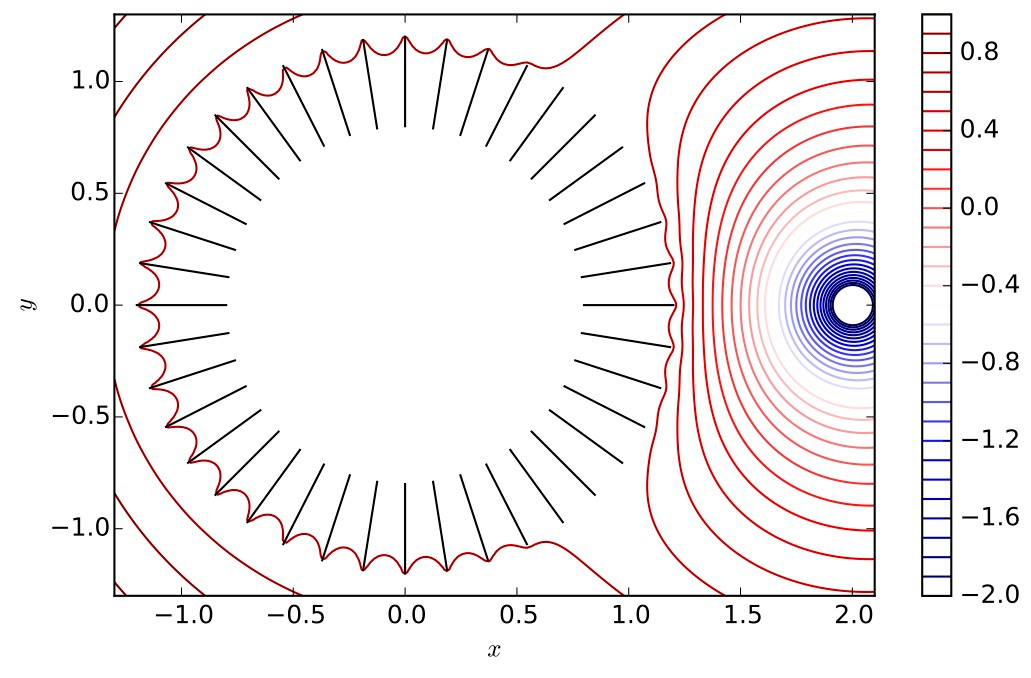
\includegraphics[width=0.67\linewidth]{Laplacetangentialplot.pdf}}
%\begin{figure}
%\centering
%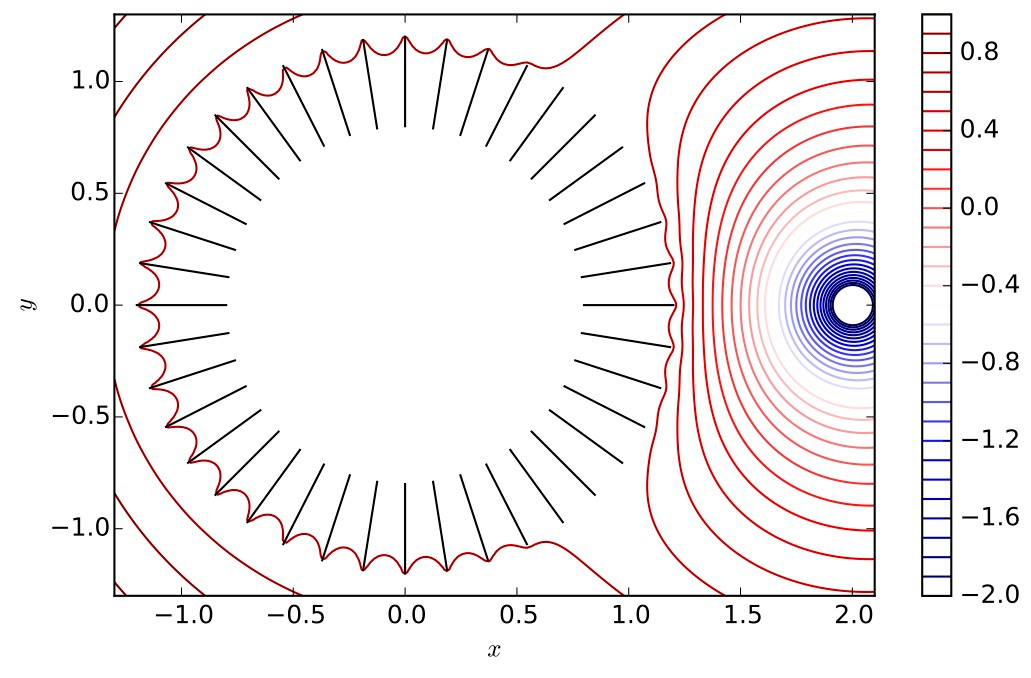
\includegraphics{Laplacetangentialplot.pdf}
%\caption{Faradaycage}
%\end{figure}


\subsection{Logarithmic singular integrals}
From the Green's function of the Laplacian, it is natural to consider logarithmic singular integrals over a contour

\[
L_\gamma f(z) = {1 \over \pi} \int_\gamma f(\zeta) \log|\zeta-z| \D s
\]
where $\D s$ is the arclength differential (as in line integrals, not complex analysis) and $f$ is real-valued. We focus on intervals where the arclength differential is just the standard one:

\[
L_{a,b} f(z) = {1 \over \pi }\int_a^b f(t) \log | z - t| \dt
\]
Note that off $[a,b]$, $u(x,y) \equiv u(x+\I y) = L f(x+\I y)$ solves Laplace's equation, and as the integrand has an integrable singularity it is continuous on $[a,b]$:


\begin{lstlisting}
(*@\HLJLk{using}@*) (*@\HLJLn{ApproxFun}@*)(*@\HLJLp{,}@*) (*@\HLJLn{SingularIntegralEquations}@*)(*@\HLJLp{,}@*) (*@\HLJLn{Plots}@*)
(*@\HLJLn{t}@*) (*@\HLJLoB{=}@*) (*@\HLJLnf{Fun}@*)(*@\HLJLp{()}@*)
(*@\HLJLn{f}@*) (*@\HLJLoB{=}@*) (*@\HLJLnf{sqrt}@*)(*@\HLJLp{(}@*)(*@\HLJLni{1}@*)(*@\HLJLoB{-}@*)(*@\HLJLn{t}@*)(*@\HLJLoB{{\textasciicircum}}@*)(*@\HLJLni{2}@*)(*@\HLJLp{)}@*)(*@\HLJLoB{*}@*)(*@\HLJLnf{exp}@*)(*@\HLJLp{(}@*)(*@\HLJLn{t}@*)(*@\HLJLp{)}@*)
(*@\HLJLn{u}@*) (*@\HLJLoB{=}@*) (*@\HLJLn{z}@*) (*@\HLJLoB{->}@*) (*@\HLJLnf{logkernel}@*)(*@\HLJLp{(}@*)(*@\HLJLn{f}@*)(*@\HLJLp{,}@*) (*@\HLJLn{z}@*)(*@\HLJLp{)}@*)  (*@\HLJLcs{{\#}}@*) (*@\HLJLcs{logkernel(f,z)}@*) (*@\HLJLcs{calculates}@*) (*@\HLJLcs{1/\ensuremath{\pi}}@*) (*@\HLJLcs{*}@*) (*@\HLJLcs{{\textbackslash}int}@*) (*@\HLJLcs{f(t)*log|t-z|}@*) (*@\HLJLcs{dt}@*)

(*@\HLJLn{xx}@*) (*@\HLJLoB{=}@*) (*@\HLJLn{yy}@*) (*@\HLJLoB{=}@*) (*@\HLJLoB{-}@*)(*@\HLJLni{2}@*)(*@\HLJLoB{:}@*)(*@\HLJLnfB{0.01}@*)(*@\HLJLoB{:}@*)(*@\HLJLni{2}@*)
(*@\HLJLn{U}@*) (*@\HLJLoB{=}@*) (*@\HLJLn{u}@*)(*@\HLJLoB{.}@*)(*@\HLJLp{(}@*)(*@\HLJLn{xx}@*)(*@\HLJLoB{{\textquotesingle}}@*) (*@\HLJLoB{.+}@*) (*@\HLJLn{im}@*)(*@\HLJLoB{*}@*)(*@\HLJLn{yy}@*)(*@\HLJLp{)}@*)

(*@\HLJLnf{contour}@*)(*@\HLJLp{(}@*)(*@\HLJLn{xx}@*)(*@\HLJLp{,}@*) (*@\HLJLn{yy}@*)(*@\HLJLp{,}@*) (*@\HLJLn{U}@*)(*@\HLJLp{)}@*)
(*@\HLJLnf{plot!}@*)(*@\HLJLp{(}@*)(*@\HLJLnf{domain}@*)(*@\HLJLp{(}@*)(*@\HLJLn{t}@*)(*@\HLJLp{);}@*) (*@\HLJLn{color}@*)(*@\HLJLoB{=:}@*)(*@\HLJLn{black}@*)(*@\HLJLp{,}@*) (*@\HLJLn{label}@*)(*@\HLJLoB{=}@*)(*@\HLJLs{"{}contour"{}}@*)(*@\HLJLp{)}@*)
\end{lstlisting}

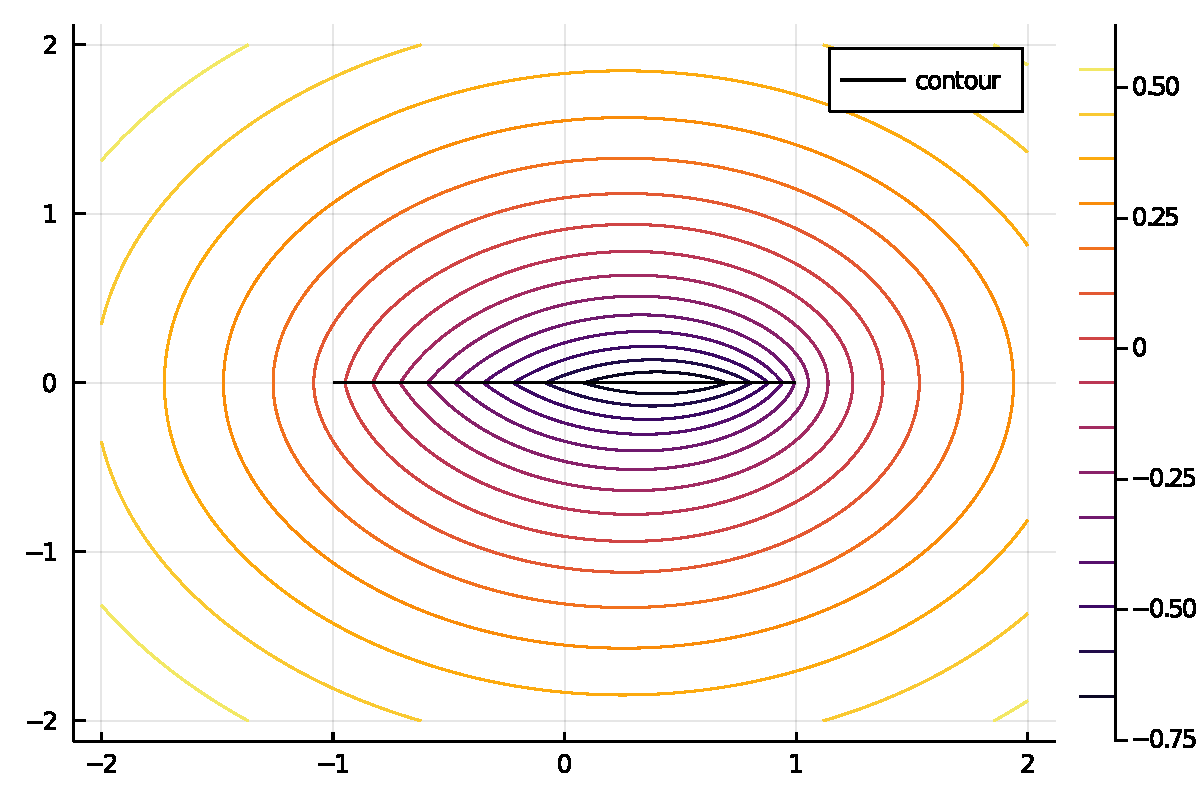
\includegraphics[width=\linewidth]{C:/Users/mfaso/OneDrive/Documents/GitHub/M3M6AppliedComplexAnalysis/output/figures/Lecture16_1_1.pdf}

Or this can also be seen from a surface plot:


\begin{lstlisting}
(*@\HLJLnf{surface}@*)(*@\HLJLp{(}@*)(*@\HLJLn{xx}@*)(*@\HLJLp{,}@*) (*@\HLJLn{yy}@*)(*@\HLJLp{,}@*) (*@\HLJLn{U}@*)(*@\HLJLp{)}@*)
\end{lstlisting}

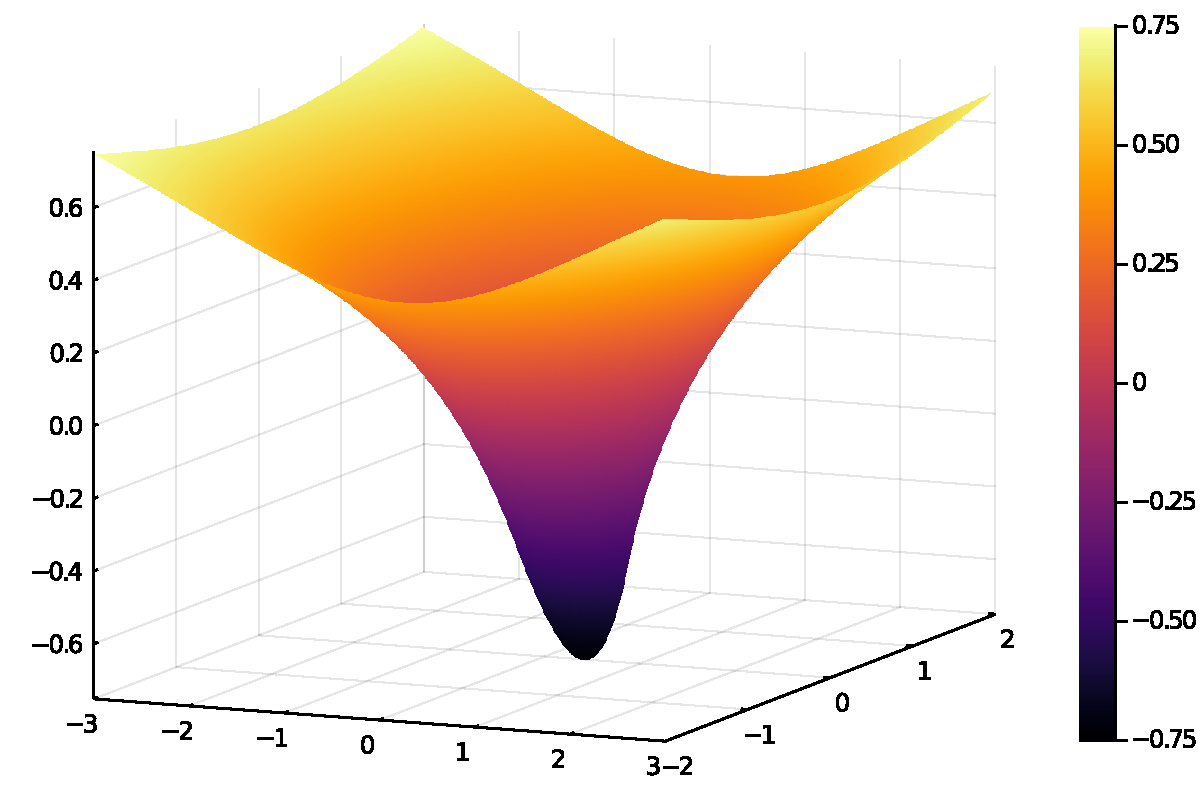
\includegraphics[width=\linewidth]{C:/Users/mfaso/OneDrive/Documents/GitHub/M3M6AppliedComplexAnalysis/output/figures/Lecture16_2_1.pdf}

For $z \notin (-\infty,b]$ the fact that $u$ is harmonic (solves Laplace's equation) can also be seen since $u$ is the real part of an analytic function:

\[
    u(z) = \Re Mf(z) \qqfor  Mf(z) := {1 \over \pi} \int_a^b f(t) \log ( z - t) \dt
\]
Note that the integrand avoids the branch cut of $\log z$. To extend this to $z\in (-\infty,a]$ (or more generally, $z \notin [a,\infty)$), we can use the alternative expression

\[
    u(z) = \Re \tilde Mf(z) \qqfor  \tilde Mf(z) := {1 \over \pi} \int_a^b f(t) \log ( t-z) \dt
\]
which follows from $\log|z-t| = \log|t-z|$.
\newpage
\subsection{Evaluating logarithmic singular integrals}
To evaluate $L f(z)$ we evaluate $M f(z)$. Following our claim that the right way to represent analytic functions is by their behaviour at singularitites/branch cuts, we will accomplish this this by investigating the jumps of $M f(z)$. This allows us to reduce it to computing a Cauchy transform.

\textbf{Lemma (Jumps of $M$)} Suppose $f$ satisfies the conditions of Plemelj. Then $M f(z)$ satisfies the following

\begin{itemize}
\item[1. ] Analyticity: $M$ is analytic off $(-\infty,b]$


\item[2. ] Regularity: $M$ has weaker than pole singularities


\item[3. ] Asymptotics:

\end{itemize}
\[
Mf(z) = {1 \over \pi} \int_a^b f(t) \D t \log z + o(1) \qqas z \rightarrow \infty
\]
\begin{itemize}
\item[4. ] Jump: for $x < a$ we have

\end{itemize}
\[
M^+f(x) - M^-f(x) = 2 \I \int_a^b f(t) \D t
\]
and for $a < x < b$ we have

\[
M^+ f(x) - M^-f(x) = 2 \I \int_x^b f(t) \D t
\]
\textbf{Proof}

Analyticity property (1) follows immediately from definition: we have for $z \notin (-\infty,b]$

\[
{\D \over \D z} M f(z) = {1 \over \pi} \int_{a}^b f(t) {1\over z -t}  \dt = -2 \I \CC_{[a,b]} f(z)
\]
The regularity property (2) follows from the expression as an antiderivative: we know $\CC f(z)$ has weaker than pole singularities and integrating only makes them better. To derive the asymptotics (3) we use

\[
\log(z - t) = \log z + \log(1 - t/z)
\]
\newpage
Finally we get to the jumps. For any point $c > b$ we write

\[
M f(z) = -2 \I \int_c^z \CC f(\zeta) \D \zeta + M f(c)
\]
For $x < a$ we can deform the contour just above/below the interval giving us

\[
M^\pm f(x) = Mf(c) -2 \I \int_c^b \CC f(t) \D t -2 \I \int_b^a \CC^\pm f(t) \D t -2 \I \int_a^x \CC f(t) \D t
\]
so that

\[
(M^+ - M^-) f(x) = -2 \I \int_b^a (\CC^+ - \CC^-) f(t) \D t  = 2 \I \int_a^b f(t) \D t
\]
Similarly for $a < x < b$ we have

\[
M^\pm f(x) = Mf(c) -2 \I \int_c^b \CC f(t) \D t -2 \I \int_b^x \CC^\pm f(t) \D t
\]
which gives

\[
(M^+ - M^-) f(x) = -2 \I \int_b^x (\CC^+ - \CC^-) f(t) \D t  = 2 \I \int_x^b f(t) \D t.
\]
\ensuremath{\blacksquare}
\newpage
We can construct a function that satisfies the same 4 properties using the Cauchy transform. By uniqueness they must be the same.

\textbf{Theorem (Log kernel as Cauchy)} Suppose $f$ satisfies the conditions of Plemelj and define the (negative) indefinite integral of $f$ via

\[
F(x) := \int_x^b f(t) \D t.
\]
Then

\[
M f(z) = {\log(z-a) \over \pi} \int_a^b f(t) \D t + 2 \I \CC_{[a,b]} F(z)
\]
\textbf{Proof}

Define

\[
\phi(z) := {\log(z-a) \over \pi} \int_a^b f(t) \D t + 2 \I \CC_{[a,b]} F(z)
\]
This satisfies conditions (1\ensuremath{\endash}4) above. Therefore $\phi(z) - M f(z)$ is continuous hence analytic on $(-\infty,a)$ and $(a,b)$, has weaker than pole singularities at $a$ and $b$ so analytic there too: it is entire. The logarithmic growth at infinity cancels therefore it is zero by Liouville.

\ensuremath{\blacksquare}

\subsection{Examples of logarithmic singular integrals}
We look at 3 examples of computing logarithmic singular integrals: $x/\sqrt{1-x^2}$, $1$, and $1/\sqrt{1-x^2}$

\subsubsection{Example 1}
Consider $f(x) = x/\sqrt{1-x^2}$ and we want to compute

\[
L f(z) = {1 \over \pi} \int_{-1}^1 {t \over \sqrt{1-t^2}} \log|t-z| \D t = \Re \underbrace{{1 \over \pi} \int_{-1}^1 {t \over \sqrt{1-t^2}} \log(z-t) \D t }_{M f(z)}
\]
We have

\[
{\D \over \dx} \sqrt{1-x^2} = - f(x)
\]
hence

\[
F(x) = \int_x^1 f(t) \D t = \sqrt{1-x^2}.
\]
and in particular $F(-1) = 0$. Recall that

\[
\CC F(z) = {\sqrt{z-1} \sqrt{z+1} - z\over 2 \I}
\]
Thus the result from last lecture gives

\[
M f(z) = {1 \over \pi} \int_{-1}^1 f(t) \D t \log(z+1)+ 2 \I \CC F(z) = \sqrt{z-1} \sqrt{z+1} - z
\]
Let's double check the formula:


\begin{lstlisting}
(*@\HLJLk{using}@*) (*@\HLJLn{ApproxFun}@*)(*@\HLJLp{,}@*) (*@\HLJLn{SingularIntegralEquations}@*)(*@\HLJLp{,}@*) (*@\HLJLn{Plots}@*)
(*@\HLJLn{x}@*) (*@\HLJLoB{=}@*) (*@\HLJLnf{Fun}@*)(*@\HLJLp{()}@*)
(*@\HLJLn{f}@*) (*@\HLJLoB{=}@*) (*@\HLJLn{x}@*)(*@\HLJLoB{/}@*)(*@\HLJLnf{sqrt}@*)(*@\HLJLp{(}@*)(*@\HLJLni{1}@*)(*@\HLJLoB{-}@*)(*@\HLJLn{x}@*)(*@\HLJLoB{{\textasciicircum}}@*)(*@\HLJLni{2}@*)(*@\HLJLp{)}@*)
(*@\HLJLn{Mf}@*) (*@\HLJLoB{=}@*) (*@\HLJLn{z}@*) (*@\HLJLoB{->}@*) (*@\HLJLnf{sqrt}@*)(*@\HLJLp{(}@*)(*@\HLJLn{z}@*)(*@\HLJLoB{-}@*)(*@\HLJLni{1}@*)(*@\HLJLp{)}@*)(*@\HLJLnf{sqrt}@*)(*@\HLJLp{(}@*)(*@\HLJLn{z}@*)(*@\HLJLoB{+}@*)(*@\HLJLni{1}@*)(*@\HLJLp{)}@*) (*@\HLJLoB{-}@*) (*@\HLJLn{z}@*)
(*@\HLJLn{Lf}@*) (*@\HLJLoB{=}@*) (*@\HLJLn{z}@*) (*@\HLJLoB{->}@*) (*@\HLJLnf{real}@*)(*@\HLJLp{(}@*)(*@\HLJLnf{Mf}@*)(*@\HLJLp{(}@*)(*@\HLJLn{z}@*)(*@\HLJLp{))}@*)
(*@\HLJLn{z}@*) (*@\HLJLoB{=}@*) (*@\HLJLnfB{0.1}@*)(*@\HLJLoB{+}@*)(*@\HLJLnfB{0.1}@*)(*@\HLJLn{im}@*)
(*@\HLJLnf{logkernel}@*)(*@\HLJLp{(}@*)(*@\HLJLn{f}@*)(*@\HLJLp{,}@*)(*@\HLJLn{z}@*)(*@\HLJLp{),}@*)(*@\HLJLnf{Lf}@*)(*@\HLJLp{(}@*)(*@\HLJLn{z}@*)(*@\HLJLp{)}@*)
\end{lstlisting}

\begin{lstlisting}
(-0.09000049991252067, -0.09000049991252063)
\end{lstlisting}


Here is a plot of the solution:


\begin{lstlisting}
(*@\HLJLn{xx}@*) (*@\HLJLoB{=}@*) (*@\HLJLnf{range}@*)(*@\HLJLp{(}@*)(*@\HLJLoB{-}@*)(*@\HLJLni{3}@*)(*@\HLJLp{,}@*)(*@\HLJLni{3}@*)(*@\HLJLp{;}@*)(*@\HLJLn{length}@*)(*@\HLJLoB{=}@*)(*@\HLJLni{300}@*)(*@\HLJLp{);}@*) (*@\HLJLn{yy}@*) (*@\HLJLoB{=}@*) (*@\HLJLnf{range}@*)(*@\HLJLp{(}@*)(*@\HLJLoB{-}@*)(*@\HLJLni{2}@*)(*@\HLJLp{,}@*)(*@\HLJLni{2}@*)(*@\HLJLp{;}@*)(*@\HLJLn{length}@*)(*@\HLJLoB{=}@*)(*@\HLJLni{200}@*)(*@\HLJLp{)}@*)
(*@\HLJLn{Z}@*) (*@\HLJLoB{=}@*) (*@\HLJLn{Lf}@*)(*@\HLJLoB{.}@*)(*@\HLJLp{(}@*)(*@\HLJLn{xx}@*)(*@\HLJLoB{{\textquotesingle}}@*) (*@\HLJLoB{.+}@*) (*@\HLJLn{im}@*)(*@\HLJLoB{*}@*)(*@\HLJLn{yy}@*)(*@\HLJLp{)}@*)
(*@\HLJLnf{contour}@*)(*@\HLJLp{(}@*)(*@\HLJLn{xx}@*)(*@\HLJLp{,}@*)(*@\HLJLn{yy}@*)(*@\HLJLp{,}@*)(*@\HLJLn{Z}@*)(*@\HLJLp{;}@*)(*@\HLJLn{ratio}@*)(*@\HLJLoB{=}@*)(*@\HLJLnfB{1.0}@*)(*@\HLJLp{)}@*)
(*@\HLJLnf{plot!}@*)(*@\HLJLp{(}@*)(*@\HLJLoB{-}@*)(*@\HLJLnfB{1..1}@*)(*@\HLJLp{;}@*) (*@\HLJLn{color}@*)(*@\HLJLoB{=:}@*)(*@\HLJLn{black}@*)(*@\HLJLp{,}@*) (*@\HLJLn{label}@*)(*@\HLJLoB{=}@*)(*@\HLJLs{"{}contour"{}}@*)(*@\HLJLp{)}@*)
\end{lstlisting}

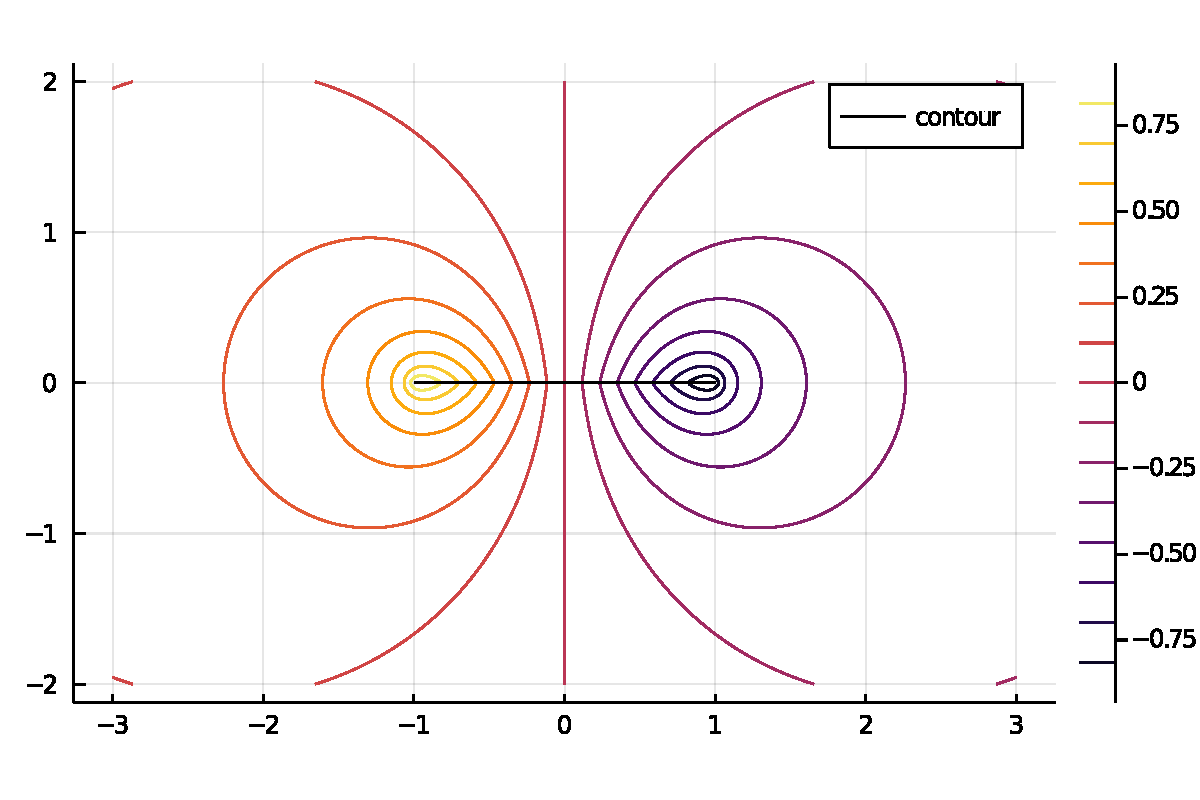
\includegraphics[width=\linewidth]{C:/Users/mfaso/OneDrive/Documents/GitHub/M3M6AppliedComplexAnalysis/output/figures/Lecture16_4_1.pdf}

\subsubsection{Example 2}
Consider $f(x) = 1$ and we want to compute

\[
L f(z) = {1 \over \pi} \int_{-1}^1 \log|t-z| \D t = \Re \underbrace{{1 \over \pi} \int_{-1}^1 \log(z-t) \D t }_{M f(z)}
\]
We have

\[
F(x) = \int_x^1 f(t) \D t = 1-x.
\]
We can determine the Cauchy transform by considering $1-z$ times the known Cauchy transform

\[
\CC 1(z) = {\log(z-1) - \log(z+1) \over 2 \pi \I} = {\I  \over  \pi z} + O(z^{-3})
\]
so that

\[
\CC F(z) =  (1-z) {\log(z-1) - \log(z+1) \over 2 \pi \I} + {\I \over \pi}
\]
Thus the result from last lecture gives


\begin{align*}
\hspace*{-0.7cm} M 1(z) &= {1 \over \pi} \int_{-1}^1  \D t \log(z+1)+ 2 \I \CC F(z) = {2 \over \pi} \log(z+1) +
(1-z) {\log(z-1) - \log(z+1) \over \pi} - {2 \over \pi} \\
&= {(1-z) \log(z-1) + (1+z) \log(z+1) -2 \over \pi}
\end{align*}
For $-1 < x < 1$ real this gives a particularly simple formula:

\[
L 1(x) = \Re M^+ 1(x) = {(1-x) \log(1-x) + (1+x)\log(x+1) - 2\over \pi}
\]
We can double check this:


\begin{lstlisting}
(*@\HLJLn{f}@*) (*@\HLJLoB{=}@*) (*@\HLJLnf{Fun}@*)(*@\HLJLp{(}@*)(*@\HLJLni{1}@*)(*@\HLJLp{,}@*)(*@\HLJLoB{-}@*)(*@\HLJLnfB{1..1}@*)(*@\HLJLp{)}@*)
(*@\HLJLn{x}@*) (*@\HLJLoB{=}@*) (*@\HLJLnfB{0.1}@*)
(*@\HLJLnf{logkernel}@*)(*@\HLJLp{(}@*)(*@\HLJLn{f}@*)(*@\HLJLp{,}@*)(*@\HLJLn{x}@*)(*@\HLJLp{),}@*) (*@\HLJLp{((}@*)(*@\HLJLni{1}@*)(*@\HLJLoB{-}@*)(*@\HLJLn{x}@*)(*@\HLJLp{)}@*)(*@\HLJLoB{*}@*)(*@\HLJLnf{log}@*)(*@\HLJLp{(}@*)(*@\HLJLni{1}@*)(*@\HLJLoB{-}@*)(*@\HLJLn{x}@*)(*@\HLJLp{)}@*) (*@\HLJLoB{+}@*) (*@\HLJLp{(}@*)(*@\HLJLni{1}@*)(*@\HLJLoB{+}@*)(*@\HLJLn{x}@*)(*@\HLJLp{)}@*)(*@\HLJLoB{*}@*)(*@\HLJLnf{log}@*)(*@\HLJLp{(}@*)(*@\HLJLn{x}@*)(*@\HLJLoB{+}@*)(*@\HLJLni{1}@*)(*@\HLJLp{)}@*) (*@\HLJLoB{-}@*) (*@\HLJLni{2}@*)(*@\HLJLp{)}@*)(*@\HLJLoB{/}@*)(*@\HLJLn{\ensuremath{\pi}}@*)
\end{lstlisting}

\begin{lstlisting}
(-0.6334313470059203, -0.6334313470059203)
\end{lstlisting}


Here is a plot of the solution:


\begin{lstlisting}
(*@\HLJLn{Lf}@*) (*@\HLJLoB{=}@*) (*@\HLJLn{z}@*) (*@\HLJLoB{->}@*) (*@\HLJLnf{real}@*)(*@\HLJLp{((}@*)(*@\HLJLni{1}@*)(*@\HLJLoB{-}@*)(*@\HLJLn{z}@*)(*@\HLJLp{)}@*)(*@\HLJLoB{*}@*)(*@\HLJLnf{log}@*)(*@\HLJLp{(}@*)(*@\HLJLn{z}@*)(*@\HLJLoB{-}@*)(*@\HLJLni{1}@*)(*@\HLJLp{)}@*) (*@\HLJLoB{+}@*) (*@\HLJLp{(}@*)(*@\HLJLni{1}@*)(*@\HLJLoB{+}@*)(*@\HLJLn{z}@*)(*@\HLJLp{)}@*)(*@\HLJLoB{*}@*)(*@\HLJLnf{log}@*)(*@\HLJLp{(}@*)(*@\HLJLn{z}@*)(*@\HLJLoB{+}@*)(*@\HLJLni{1}@*)(*@\HLJLp{)}@*) (*@\HLJLoB{-}@*) (*@\HLJLni{2}@*)(*@\HLJLp{)}@*)(*@\HLJLoB{/}@*)(*@\HLJLn{\ensuremath{\pi}}@*)
(*@\HLJLn{Z}@*) (*@\HLJLoB{=}@*) (*@\HLJLn{Lf}@*)(*@\HLJLoB{.}@*)(*@\HLJLp{(}@*)(*@\HLJLn{xx}@*)(*@\HLJLoB{{\textquotesingle}}@*) (*@\HLJLoB{.+}@*) (*@\HLJLn{im}@*)(*@\HLJLoB{*}@*)(*@\HLJLn{yy}@*)(*@\HLJLp{)}@*)
(*@\HLJLnf{contour}@*)(*@\HLJLp{(}@*)(*@\HLJLn{xx}@*)(*@\HLJLp{,}@*)(*@\HLJLn{yy}@*)(*@\HLJLp{,}@*)(*@\HLJLn{Z}@*)(*@\HLJLp{;}@*)(*@\HLJLn{ratio}@*)(*@\HLJLoB{=}@*)(*@\HLJLnfB{1.0}@*)(*@\HLJLp{)}@*)
(*@\HLJLnf{plot!}@*)(*@\HLJLp{(}@*)(*@\HLJLoB{-}@*)(*@\HLJLnfB{1..1}@*)(*@\HLJLp{;}@*) (*@\HLJLn{color}@*)(*@\HLJLoB{=:}@*)(*@\HLJLn{black}@*)(*@\HLJLp{,}@*) (*@\HLJLn{label}@*)(*@\HLJLoB{=}@*)(*@\HLJLs{"{}contour"{}}@*)(*@\HLJLp{)}@*)
\end{lstlisting}

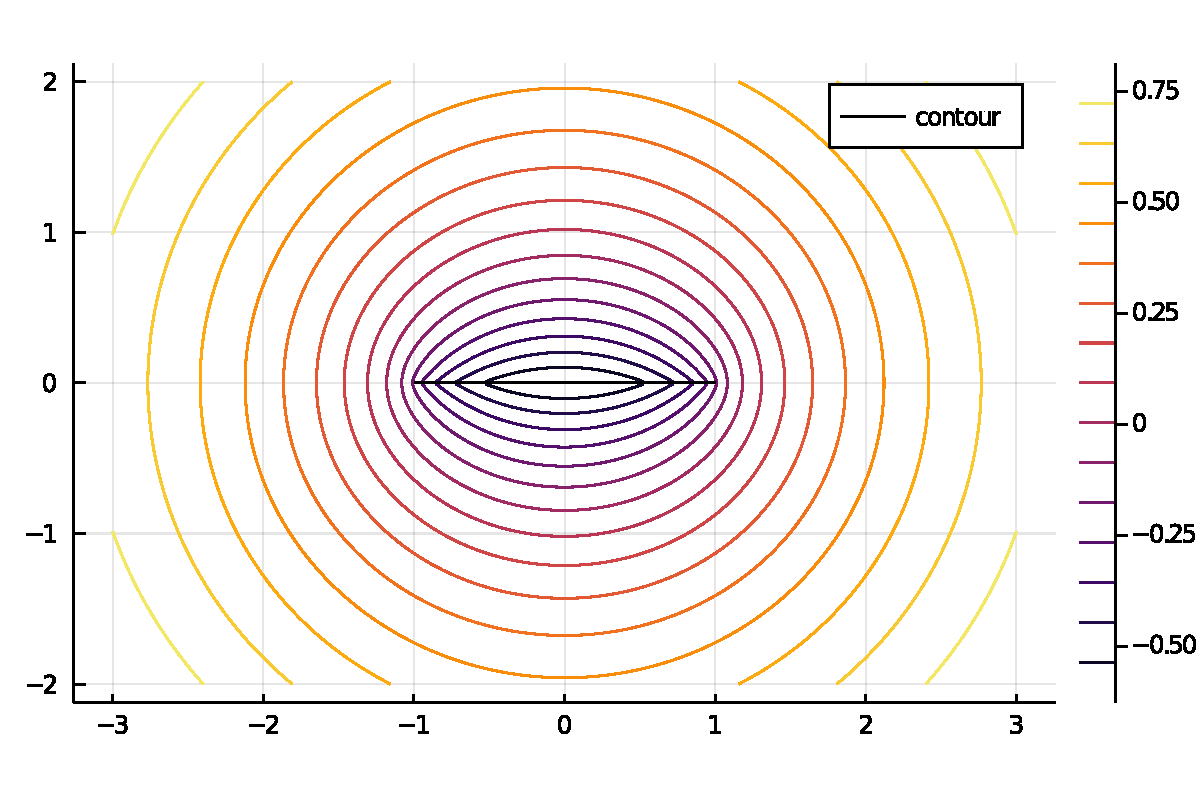
\includegraphics[width=\linewidth]{C:/Users/mfaso/OneDrive/Documents/GitHub/M3M6AppliedComplexAnalysis/output/figures/Lecture16_6_1.pdf}

\subsubsection{Example 3}
Consider $f(x) = 1/\sqrt{1-x^2}$. We have

\[
F(x) = \acos x = 2 \atan {\sqrt{1-x} \over \sqrt{1+x}}
\]
where the second version can be verified by differentiation, using $\atan' x = 1/(1+x^2)$. One can determine $M$ by indefinite integration of

\[
\CC f(z) = {\I \over 2 \sqrt{z-1}\sqrt{z+1}}
\]
but we prefer to start with an ansatz and verify the solution. Namely, consider

\[
\phi(z) := {\log(\sqrt{z-1} + \sqrt{z+1}) \over \I}.
\]
First, this is analytic off $(-\infty,1]$, as for $z$ in the upper-half plane we have $\sqrt{z-1}$ and $\sqrt{z+1}$ are  in the upper-right quadrant: we never cross the branch cut of $\log z$. Similar argument holds for $z$ in the lower-half plane. On $x \in (-\infty,-1]$ it has the jump


\begin{align*}
\phi_+(x) - \phi_-(x) &= {\log(\I (\sqrt{1-x} + \sqrt{-x-1})) -  \log(-\I (\sqrt{1-x} + \sqrt{-x-1})) \over \I} \\
& =
        2 \arg(\I (\sqrt{1-x} + \sqrt{-x-1})) = \pi
\end{align*}
For $x \in (-1,1)$ we have


\begin{align*}
\phi_+(x) - \phi_-(x) &= {\log(\I \sqrt{1-x} + \sqrt{1-x}) -  \log(-\I \sqrt{1-x} + \sqrt{1-x}) \over \I} \\
& =
        2 \arg(\I \sqrt{1-x} + \sqrt{-x-1}) = 2 \atan {\sqrt{1-x} \over \sqrt{1+x}} = F(x).
\end{align*}
Finally we have

\[
\phi(z) = {\log z \over 2 \I} - \I \log 2 + o(1)
\]
We therefore have from Plemelj that

\[
\CC F(z) = \phi(z) - {\log(z+1) \over 2 \I} + \I \log 2
\]
and

\[
Mf(z) = {F(-1)\over \pi} \log(z+1)  + 2 \I \CC F(z) =2\log(\sqrt{z-1} + \sqrt{z+1}) -2 \log 2
\]
Here is a plot of the solution:


\begin{lstlisting}
(*@\HLJLn{Lf}@*) (*@\HLJLoB{=}@*) (*@\HLJLn{z}@*) (*@\HLJLoB{->}@*) (*@\HLJLnf{real}@*)(*@\HLJLp{(}@*)(*@\HLJLni{2}@*)(*@\HLJLnf{log}@*)(*@\HLJLp{(}@*)(*@\HLJLnf{sqrt}@*)(*@\HLJLp{(}@*)(*@\HLJLn{z}@*)(*@\HLJLoB{-}@*)(*@\HLJLni{1}@*)(*@\HLJLp{)}@*) (*@\HLJLoB{+}@*) (*@\HLJLnf{sqrt}@*)(*@\HLJLp{(}@*)(*@\HLJLn{z}@*)(*@\HLJLoB{+}@*)(*@\HLJLni{1}@*)(*@\HLJLp{))}@*) (*@\HLJLoB{-}@*) (*@\HLJLni{2}@*)(*@\HLJLnf{log}@*)(*@\HLJLp{(}@*)(*@\HLJLni{2}@*)(*@\HLJLp{))}@*)
(*@\HLJLn{Z}@*) (*@\HLJLoB{=}@*) (*@\HLJLn{Lf}@*)(*@\HLJLoB{.}@*)(*@\HLJLp{(}@*)(*@\HLJLn{xx}@*)(*@\HLJLoB{{\textquotesingle}}@*) (*@\HLJLoB{.+}@*) (*@\HLJLn{im}@*)(*@\HLJLoB{*}@*)(*@\HLJLn{yy}@*)(*@\HLJLp{)}@*)
(*@\HLJLnf{contour}@*)(*@\HLJLp{(}@*)(*@\HLJLn{xx}@*)(*@\HLJLp{,}@*)(*@\HLJLn{yy}@*)(*@\HLJLp{,}@*)(*@\HLJLn{Z}@*)(*@\HLJLp{;}@*)(*@\HLJLn{ratio}@*)(*@\HLJLoB{=}@*)(*@\HLJLnfB{1.0}@*)(*@\HLJLp{)}@*)
(*@\HLJLnf{plot!}@*)(*@\HLJLp{(}@*)(*@\HLJLoB{-}@*)(*@\HLJLnfB{1..1}@*)(*@\HLJLp{;}@*) (*@\HLJLn{color}@*)(*@\HLJLoB{=:}@*)(*@\HLJLn{black}@*)(*@\HLJLp{,}@*) (*@\HLJLn{label}@*)(*@\HLJLoB{=}@*)(*@\HLJLs{"{}contour"{}}@*)(*@\HLJLp{)}@*)
\end{lstlisting}

\cent{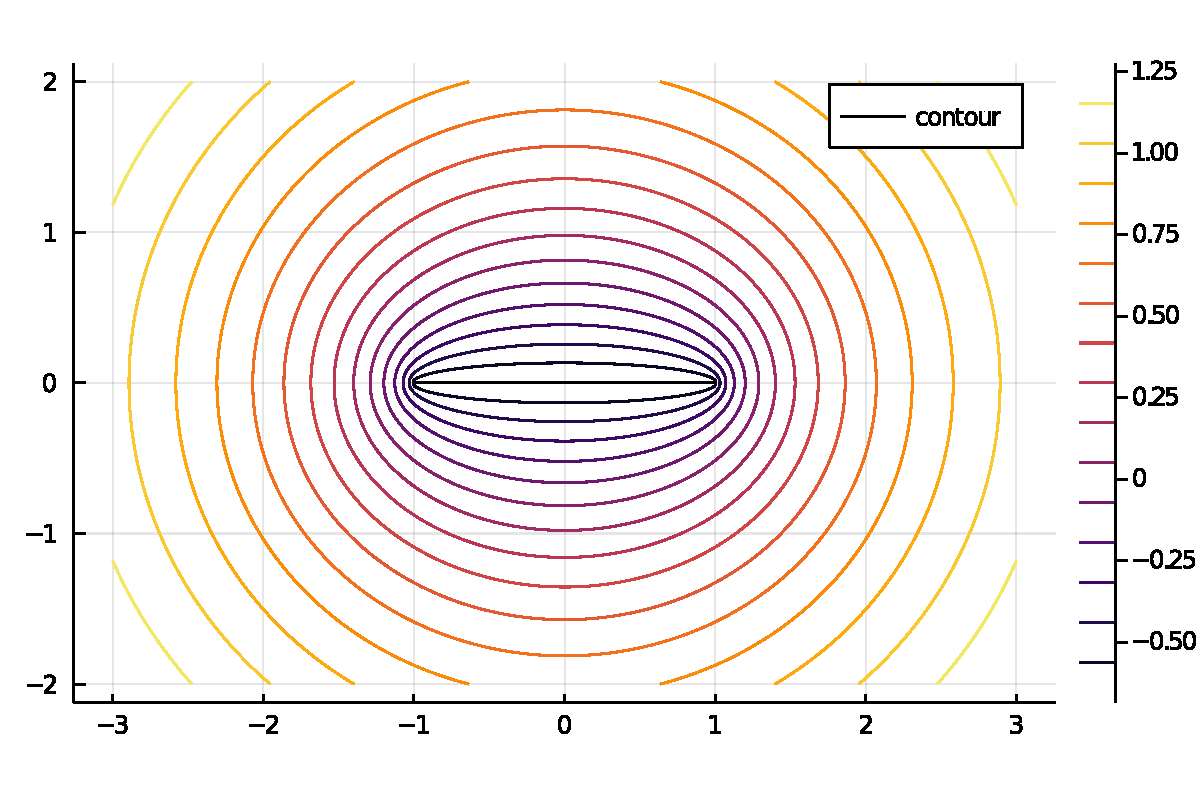
\includegraphics[width=0.925\linewidth]{C:/Users/mfaso/OneDrive/Documents/GitHub/M3M6AppliedComplexAnalysis/output/figures/Lecture16_7_1.pdf}}
Note that it is clearly visible that it is constant on the contour, which follows from:
\begin{align*}
L f(x)& = \Re M f(x) = 2\Re \log(\I \sqrt{1-x} + \sqrt{1+x}) -2 \log 2 = 2 \log\sqrt{1-x+1+x} - 2 \log 2 \\
& = - \log 2
\end{align*}

}
\end{document}
